\section{Connection operations}\label{sec:connections}

We now construct closed walks that touch existing layers at a cost charged to specified period budgets. We first give joins paid for entirely by the layers being attached, then an operation that also spends the receiving layer's budget. Each cross-text contact uses an actual word common to the two alignments; the band operation below is restricted to layers of one primitive-text group.

A collection of layers and added walks is \emph{rooted} if its graph support is connected to $\eps$. Connectivity is in the underlying undirected graph; every edge multiset we use is balanced. To \emph{touch} a layer means to share at least one of its graph vertices. Since all base edges remain, touching any vertex of a layer connects to every vertex of that layer.

\subsection{Following ordered windows}

\begin{lemma}[Ordered windows]\label{lem:ordered-windows}
Let $[a,b)$ and $[c,d)$ be windows in a common text over $\Sigma$, each spelling a word in $V$. If $a\le c$ and $b\le d$, there is a hierarchical-graph walk from the first word to the second of cost $d-b$. It visits a word of length at most $\max(0,b-c)$.

Consequently an ordered list of windows, with both starts and ends nondecreasing, can be followed at cost equal to the total increase in its ends. If its last window is a translate of the first by $h$ in a text of period dividing $h$, this is a closed walk of cost $h$.
\end{lemma}

\begin{proof}
If $c\le b$, delete the first $c-a$ letters, reaching $[c,b)$, and append through $d$. The words on the down path are suffixes of the first word; those on the up path are prefixes of the second. All belong to $V$, and the up cost is $d-b$.

If $c>b$, delete to the empty word. For each letter in the gap $[b,c)$, take an up step to that letter and a down step back to empty. Then build $[c,d)$. Single-letter words in the gap belong to $V$ because the text uses only $\Sigma$. The cost is $(c-b)+(d-c)=d-b$. Concatenating these constructions proves the assertions about lists and translates.
\end{proof}

In particular, a round trip from a vertex $s$ to $\eps$ and back costs $\len s$. Prescribed windows, rather than all intervals they sweep across, must belong to $V$; \Cref{lem:ordered-windows} supplies the intermediate vertices.

\begin{lemma}[Joining an ordered band]\label{lem:band}
Consider $k$ ordered layers from one primitive-text group of period $p$. At a start $t$, let $H$ be the top layer's first end and $E$ the bottom layer's last end. If $h$ is a nonnegative multiple of $p$ and $H-E\le h$, the layers can be joined together by a closed walk of cost at most $h$.
\end{lemma}

\begin{proof}
If $E\ge H$, every layer contains $[t,E)$: its first end is at most $H$ and its last end is at least $E$. No added walk is needed. Otherwise grow at start $t$ from end $E$ to $H$. Every layer has a vertical range intersecting $[E,H]$, so the growth touches them all. The endpoints are actual bottom and top vertices, and every intermediate word is a prefix of the top vertex. Finish by following to $[t+h,E+h)$, which is a period translate of the starting window. Since $E+h\ge H$, \Cref{lem:ordered-windows} gives a closed walk of cost $h$.
\end{proof}

\subsection{A collective outgoing link}

We call a chosen actual layer window, together with an alignment to a specified periodic text agreeing throughout it, a \emph{record}. A record on a receiving layer provides a vertex at which to attach layers following the other text. An ordinary \emph{link} spends only the attached layers' budgets. The following link attaches $k$ source layers at combined cost $kp$; it can therefore be planned without reserving any budget of the receiving layer. \Cref{fig:collective} illustrates its construction.

\begin{lemma}[Collective link]\label{lem:collective}
Consider $k$ ordered layers with a common period-$p$ text $A$, and put $K=kp$. Let $R=[a,b)$ spell a word in $V$ agreeing with $A$. Let $r_H=f_H(a)$ be the top layer's first end and $r_L=l_L(a)$ the bottom layer's last end. If
\begin{equation}\label{eq:collective-conditions}
r_H\le b+K,\qquad r_H-r_L\le K,
\qquad r_L+K\ge b,
\end{equation}
there is a cost-$K$ closed walk based at the word of $R$ that touches all $k$ layers.
\end{lemma}

\begin{proof}
Put $Y=\max(b,r_H)$. Then $b\le Y\le b+K$. For each constituent layer $i$,
\[
f_i(a)\le Y\le l_i(a)+K=l_i(a+K).
\]
Consequently its path meets height $Y$ at a start in $[a,a+K]$. More explicitly, choose the least such start $x_i$ with $z_i(x_i)\ge Y$. If $x_i=a$, then $z_i(a-1)=f_i(a)\le Y$; otherwise minimality gives $z_i(x_i-1)<Y$. Thus $[x_i,Y)$ is an actual vertex. Pointwise layer order makes the $x_i$ nondecreasing when layers are taken from top to bottom. The list from $R$ through these vertices to $R+K$ has nondecreasing starts and ends, and it closes because $K$ is a multiple of $p$. Apply \Cref{lem:ordered-windows}.
\end{proof}

\begin{figure}[tbp]
\centering
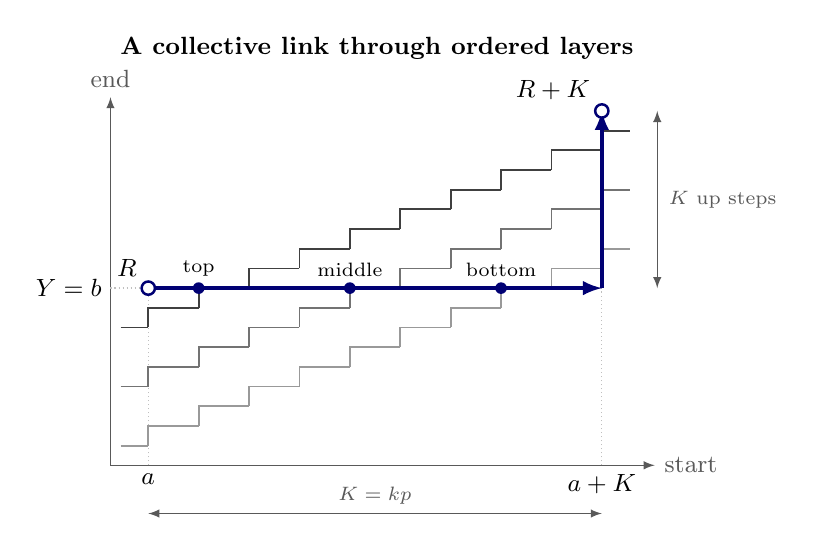
\begin{tikzpicture}[font=\small,>=latex,
  layer/.style={line width=.65pt,draw=black!55},
  connection/.style={line width=1.35pt,draw=blue!45!black},
  guide/.style={draw=black!25,densely dotted,line width=.45pt}]

  \begin{scope}[x=.64cm,y=.25cm]
    \node[anchor=west,font=\small\bfseries] at (-.75,24.2)
      {A collective link through ordered layers};
    \draw[->,black!65] (-.75,3) -- (10.05,3) node[right] {start};
    \draw[->,black!65] (-.75,3) -- (-.75,21.7) node[above] {end};
    \draw[guide] (0,3) -- (0,12);
    \draw[guide] (9,3) -- (9,12);
    \draw[guide] (-.75,12) -- (0,12);
    \node[left,inner sep=3pt] at (-.75,12) {$Y=b$};
    \node[below,inner sep=3pt] at (0,3) {$a$};
    \node[below,inner sep=3pt] at (9,3) {$a+K$};

    \foreach \c/\shade in {11/75,8/55,5/40} {
      \draw[layer,draw=black!\shade] (-.55,\c-1) -- (0,\c-1);
      \foreach \j in {0,...,8} {
        \draw[layer,draw=black!\shade]
          (\j,\j+\c-1) -- (\j,\j+\c) -- (\j+1,\j+\c);
      }
      \draw[layer,draw=black!\shade]
        (9,9+\c-1) -- (9,9+\c) -- (9.55,9+\c);
    }

    \draw[connection,->] (0,12) -- (9,12);
    \draw[connection,->] (9,12) -- (9,21);
    \foreach \j/\name in {1/top,4/middle,7/bottom} {
      \fill[blue!45!black] (\j,12) circle (2.1pt);
      \node[above,inner sep=4pt,font=\scriptsize] at (\j,12) {\name};
    }
    \filldraw[connection,fill=white,line width=.9pt] (0,12) circle (2.4pt);
    \node[above left,inner sep=4pt] at (0,12) {$R$};
    \filldraw[connection,fill=white,line width=.9pt] (9,21) circle (2.4pt);
    \node[above left,inner sep=4pt] at (9,21) {$R+K$};
    \draw[<->,black!65] (10.1,12) -- (10.1,21)
      node[midway,right,inner sep=4pt,align=left,font=\scriptsize]
      {$K$ up steps};
    \draw[<->,black!65] (0,.55) -- (9,.55)
      node[midway,above,inner sep=3pt,font=\scriptsize] {$K=kp$};
  \end{scope}
\end{tikzpicture}

\caption{A collective link in start--end coordinates. The common height $Y$ meets the ordered layers from top to bottom as the start increases. The endpoints $R$ and $R+K$ spell the same word in the source text, so the path closes at cost $K$. The illustration uses $Y=b$; the precise conditions are in \Cref{lem:collective}.}
\label{fig:collective}
\end{figure}

\subsection{Several requests at one host}

A \emph{request} reserves a source layer's budget for an operation at a receiving layer, called its \emph{host}. Unlike a link, this operation may also spend the host's budget. It handles all requests at that host together and roots every participating layer. In \Cref{sec:processing}, we will send requests only when the following hypotheses hold.

\begin{lemma}[Host requests]\label{lem:host}
Let a host layer have period $q$. On that layer choose actual windows $R_i=[a_i,b_i)$, indexed by a nonempty collection of distinct child groups. The text of child group $i$ has period $p_i$, is different up to translation from the host's text and from every other child group's text, and agrees with the host throughout $R_i$ in the chosen alignment.

For each $i$, one or more child layers request a connection at this same record. Each has a specified actual window $[a_i,e)$ satisfying
\begin{equation}\label{eq:request-condition}
a_i+p_i<e\le b_i-p_i.
\end{equation}
Its period-$p_i$ budget is reserved for the request. If the host's period-$q$ budget is also available, the host and all requesting layers can be rooted using at most these budgets.
\end{lemma}

\begin{proof}
We will spend the host budget on one closed excursion through contact words for the requesting layers. Requesters from all but one child group attach to those contacts using their own budgets. The requesters from the remaining group are touched directly by the host excursion, leaving one of their budgets to connect a contact shorter than their period to $\eps$.

By \Cref{lem:agreement},
\begin{equation}\label{eq:host-length}
b_i-a_i<p_i+q.
\end{equation}
If record $i$ is before record $l$ along a lift of the host path, their starts and ends are ordered. When $b_i>a_l$, their overlap is an agreement interval between two distinct child texts, so
\begin{equation}\label{eq:child-overlap}
b_i-a_l<p_i+p_l.
\end{equation}
If there is no overlap, the same strict inequality is immediate.

Choose an index $j$ of minimum $p_j$. Start at its record and order all other records before the next copy of it, translating coordinates by multiples of $q$ as needed. A shift by $\delta\in q\ZZ$ also transports that record's entire child coordinate system: replace its text by $A_i'(x)=A_i(x-\delta)$, its layer functions by $z_i'(x)=z_i(x-\delta)+\delta$, and its requester ends by $e+\delta$. This preserves all graph words, child periods, and budgets; the host text is unchanged because it is $q$-periodic. The same convention applies to the next copy of record $j$ when comparing overlaps. Put $T=a_j+q$. The order gives
\begin{equation}\label{eq:host-order}
a_j\le a_i\le T,\qquad b_j\le b_i\le b_j+q.
\end{equation}

To construct the host excursion, first visit all specified windows of the requesters at $j$ at start $a_j$, in increasing order of their ends $e$, and then visit $R_j$. For each later record $i$, the raw contact $[a_i+p_i,e)$ is obtained by deleting the first $p_i$ letters of the requester window and lies inside $R_i$. To place these contacts after $R_j$ and before the return at start $T$, we must keep their ends at least $b_j$ and their starts at most $T$. Accordingly, replace the raw contact by
\begin{equation}\label{eq:host-target}
Q_{i,e}=[s_i,h_{i,e})
=[\min(a_i+p_i,T),\max(e,b_j)).
\end{equation}
Visit these targets in record order and, within each record, in increasing order of $e$. Finally return to the first requester window translated by $q$.

For earlier $i$ and later $l$, \eqref{eq:request-condition} and \eqref{eq:child-overlap} give
\[
a_i+p_i<e_i\le b_i-p_i<a_l+p_l<e_l.
\]
Thus the raw targets have ordered starts and ends. The monotone operations in \eqref{eq:host-target} preserve this order. By \eqref{eq:host-order}, each modified target remains inside its record $R_i$, and it is nonempty because $s_i\le a_i+p_i<e\le h_{i,e}$. It therefore spells a word in $V$ and matches child text $i$.

Applying \eqref{eq:child-overlap} to $i$ and the next occurrence of $j$ gives
\[
b_i-T<p_i+p_j.
\]
Together with \eqref{eq:host-length}, this implies
\begin{equation}\label{eq:host-short-end}
e\le b_i-p_i<T+p_j,\qquad b_j<T+p_j,
\qquad h_{i,e}<T+p_j.
\end{equation}
If $e_0$ is the first requester end at $j$, then $e_0>a_j+p_j$, so the final translated window $[T,e_0+q)$ has end greater than $T+p_j$. The whole list is therefore ordered. Its closed excursion costs $q$ by \Cref{lem:ordered-windows}. On its final transition it reaches a vertex of length less than $p_j$. If there are no later records, the same conclusion follows using $b_j<T+p_j$.

It remains to attach the other requesters and root the piece. For a requester at $i\ne j$, the target satisfies
\begin{equation}\label{eq:target-child-range}
a_i\le s_i\le a_i+p_i,
\qquad e\le h_{i,e}\le e+p_i.
\end{equation}
Only the upper end bound needs an additional check. Here the choice of a minimum period $p_j$ is used: if $h_{i,e}=b_j$, then
\[
b_j<a_i+p_j+p_i\le a_i+2p_i<e+p_i.
\]
In child text $i$, follow the ordered list
\[
Q_{i,e},\quad[a_i+p_i,e+p_i),\quad Q_{i,e}+p_i.
\]
The middle word is a period translate of the actual requester vertex; the last word equals the first. The inequalities \eqref{eq:target-child-range} make the list ordered. Its cost-$p_i$ loop attaches this requester at the target. Do this separately for all requesters with $i\ne j$.

The requesters at $j$ were already touched in the initial vertical part, so their budgets have not been spent. Use one of their budgets $p_j$ to connect the short contact from \eqref{eq:host-short-end} to $\eps$. The host is touched at $R_j$, all requesters are attached, and the expenditure is at most the host budget plus all requester budgets.
\end{proof}
